\chapter{彭罗斯图与真实黑洞的形成}

克鲁斯卡尔图景为施瓦西视界附近区域提供了优雅的描述，但真实黑洞并非永恒存在：它是在物质坍缩时形成的。扩展图景中的哪些部分能在这一物理历史中保留下来？要回答这个问题，我们需要一幅足够大、能容纳整个时空，又足够严谨、能保持光之运动的图。我们将首先紧致化平直时空，然后紧致化施瓦西时空，最后将适当的部分跨越一个内落辐射壳层缝合起来。

\section{视界附近：克鲁斯卡尔回顾与四个象限}

我们正好从上一讲结束的地方开始。在施瓦西视界附近，几何局部看起来像平直空间。视界本身的行为类似于双曲极坐标轨迹，正如普通闵可夫斯基时空中的加速坐标那样。在这个局部图景中，我们从一开始就施加一条规则，并且从不放松它：径向光线画在\(45^\circ\)处，而每一条类时世界线都必须保持比那些零线更陡。

在这个回顾中，这些坐标最好被理解为内落观察者所看到的时间和空间。在这些局部惯性坐标中，视界附近看起来几乎是平直的。但是，一个坚持在洞外固定半径处悬停的观察者并不是惯性的。相对于内落参考系，这样的人描绘出一条加速曲线。悬停得越靠近视界，留在外面所需的加速度就越大。这就是黑板上右侧所画的那一族外部曲线的物理内容。

\begin{figure}[htbp]
\centering
\includegraphics[width=0.72\textwidth]{lecture_08_figure_02.png}
\caption{视界附近四区域几何的黑板草图。外部区域中的红色曲线记录了一族在固定半径处悬停的世界线。}
\lectureframe{00:02:54}
\end{figure}

\begin{figure}[htbp]
\centering
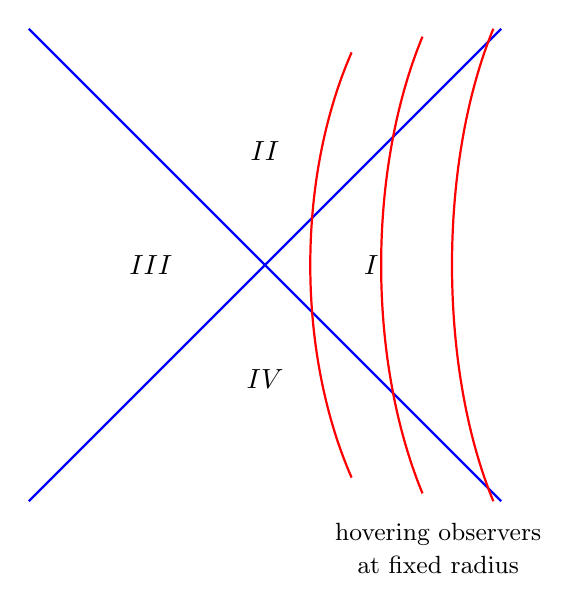
\begin{tikzpicture}[scale=1.0]
\draw[thick,blue] (-3,3) -- (3,-3);
\draw[thick,blue] (-3,-3) -- (3,3);

\draw[red,thick] (1.1,-2.7) .. controls (0.4,-1.1) and (0.4,1.1) .. (1.1,2.7);
\draw[red,thick] (2.0,-2.9) .. controls (1.3,-1.2) and (1.3,1.2) .. (2.0,2.9);
\draw[red,thick] (2.9,-3.0) .. controls (2.2,-1.3) and (2.2,1.3) .. (2.9,3.0);

\node at (1.35,0.0) {$I$};
\node at (0.0,1.45) {$II$};
\node at (-1.45,0.0) {$III$};
\node at (0.0,-1.45) {$IV$};

\node[align=center] at (2.2,-3.6) {\small hovering observers\\\small at fixed radius};
\end{tikzpicture}
\caption{回顾中所用克鲁斯卡尔式因果结构的清晰重绘。区域\(I\)是外部，区域\(II\)是不可避免的内部，而区域\(III\)和\(IV\)属于形式扩展，对于真实坍缩黑洞，这些区域稍后将被丢弃。}
\end{figure}

这已经足以说明黑洞做什么了。在外部区域\(I\)中，物体和信号可以向内运动，但它们也可以留在外面或折返向外。相比之下，在区域\(II\)中，因果裁决是固定的。一旦进入内部，就不存在回到外部的未来指向因果路径。要从区域\(II\)逃到任一外部区域，就需要在某处有一条比\(45^\circ\)更浅的轨迹，因此也就是超光速的。每一条允许的未来类时轨迹都终结于奇点。

这个开篇回顾不仅仅是重复。它为本讲的主要主题做准备。克鲁斯卡尔图景是有用的，但并非其中所有内容对真实黑洞都具有物理意义。

\begin{classroomqa}
\audiencequestion{图的坐标轴是什么，红色曲线是谁的固定位置世界线？}
\lecturerresponse{坐标轴是自由下落观察者所自然使用的坐标中的时间和空间。在视界附近，该观察者看到的是一个几乎普通的平直时空。相反，红色的恒定位置曲线属于被保持在洞外静止的观察者。它们是加速世界线，所需的加速度越靠近视界越大。
\lecturetimestamp{00:05:58--00:06:47}}
\end{classroomqa}

\section{为什么要紧致化？从无限时空到有限黑板}

下一步是方法论上的。这些图中的零方向延伸到无穷远，时间本身也是如此。因此，除非我们改变坐标，否则无法把整个时空画在普通黑板上。讲者的动机非常具体：如果我们想一下子看到一切，并推理全局因果结构，就需要一种方法，把无限时空压缩到有限区域中，同时保持光线仍然可辨认。

因此他退回到简单情形，即熟悉的平直时空。由于所关心的问题具有球对称性，我们略去角方向，只保留时间和径向坐标。我们使用坐标\(T\)和\(R\)，其中
\[
R\ge 0,
\]
因为负径向距离在极坐标中没有意义。我们还选择单位使得
\[
c=1.
\]
按照这一约定，径向零运动画在\(45^\circ\)处。

在引入紧致化映射之前，讲座花了一些时间让我们在\(T\)-\(R\)平面上定位。画出时间轴、径向轴、几条等时切片\(T=0,\pm1,\pm2\)，以及几条等半径线\(R=1,2,3\)。这并非死板的形式主义。它为我们提供了地标，并清楚地表明，当图后来被压缩到有限大小时，我们希望保留哪些特征。

关于原点，还有一个微妙但重要的教学要点。在约化径向图像中，恰好瞄准\(R=0\)的光线看起来会从原点反弹并返回。但并没有任何东西在物理上从墙壁反射。在完整的球对称几何中，光线只是穿过原点并从另一侧射出。表面上的反弹只是使用半平面\(R\ge 0\)的结果。

同样，错过原点的光线一开始看起来几乎相同，到达最近接近点，然后向外折返。在这些坐标中，它甚至可能看起来像是有什么东西把它从原点排斥开。但那同样是对熟悉的角动量势垒的坐标描述，而不是一种新的力。讲师在这些例子上停留较久，因为他希望听众在他变形图之前先信任这张图。

现在到了关键的一步。我们将要挤压和拉伸这幅图，但保持一件事固定：径向光线必须仍然是\(45^\circ\)线。这就是紧致化的全部要点。

\begin{classroomqa}
\audiencequestion{在所选择的原点处，是否有任何物理上特殊的东西，而那些看似弯曲的光线是否是那里存在力的证据？}
\lecturerresponse{没有。在这个阶段，原点仅仅是球坐标所选择的中心。表面上的反弹和弯曲来自将完整的空间运动约化为\(R\geq0\)。对称性可能使某个中心变得方便，就像对太阳那样，但坐标选择并不会在那里放置一个黑洞或一面反射墙。
\lecturetimestamp{00:16:27--00:17:08}}
\end{classroomqa}

\section{零坐标中的平直时空与彭罗斯形式}

为了使变形精确，我们引入零坐标。这是讲座中数学上干净的部分，黑板上的推导明确展示了这一步。

\begin{figure}[htbp]
\centering
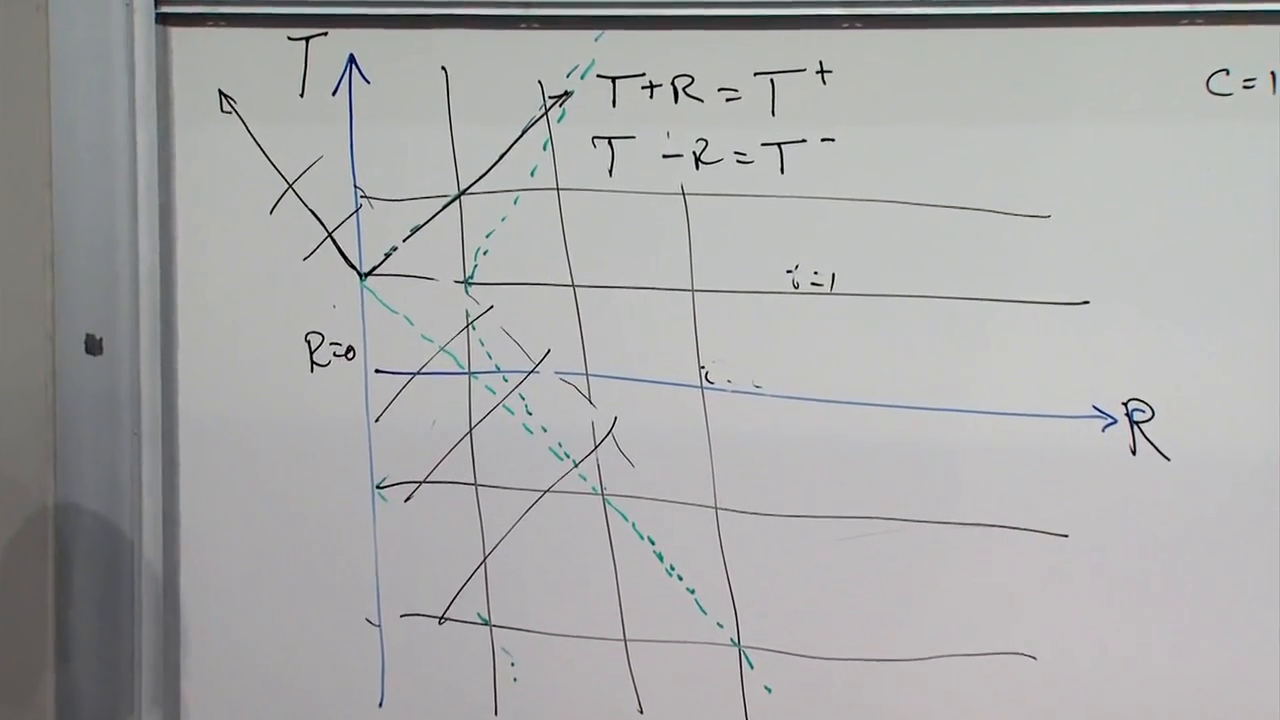
\includegraphics[width=0.82\textwidth]{lecture_08_figure_03.png}
\caption{在引入\(T^+=T+R\)和\(T^-=T-R\)时未受遮挡的\(T\)-\(R\)黑板。约化径向原点就是蓝色竖线\(R=0\)。}
\lectureframe{00:19:45}
\end{figure}

我们定义
\begin{align}
T^+ &= T+R, \\
T^- &= T-R.
\end{align}
这些坐标适用于径向零运动。入射径向光线具有\(T^+=\text{const}\)，而出射径向光线具有\(T^-=\text{const}\)。

\paragraph{推导示例。}
线\(R=0\)在这些坐标中变得特别简单。事实上，
\begin{align}
R=0
&\iff T+R=T-R \\
&\iff T^+=T^-.
\end{align}
因此整个类时边界\(R=0\)由单一关系式描述
\begin{equation}
R=0 \iff T^+=T^-.
\end{equation}

\begin{figure}[htbp]
\centering
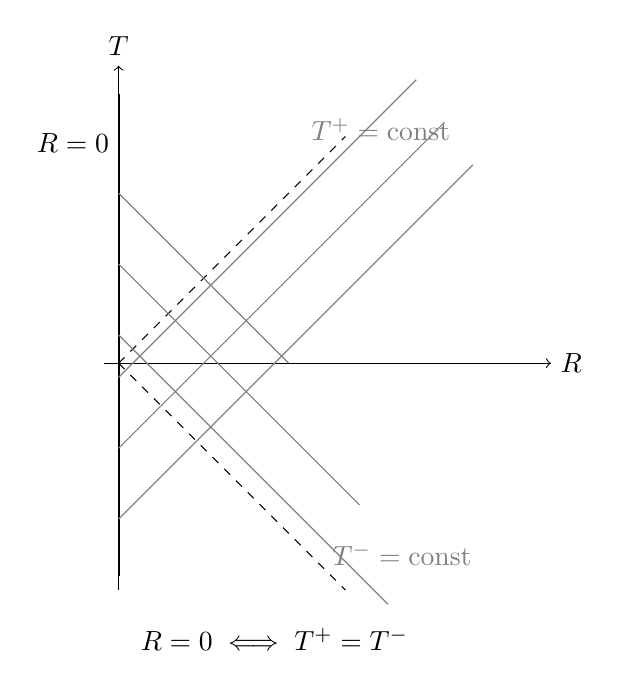
\begin{tikzpicture}[scale=0.9]
\draw[->] (-0.2,0) -- (6.1,0) node[right] {$R$};
\draw[->] (0,-3.2) -- (0,4.2) node[above] {$T$};

\draw[thick] (0,-3.0) -- (0,3.8);
\node[left] at (0,3.1) {$R=0$};

\draw[dashed] (0,0) -- (3.2,3.2);
\draw[dashed] (0,0) -- (3.2,-3.2);

\draw[gray] (0,2.4) -- (2.4,0);
\draw[gray] (0,1.4) -- (3.4,-2.0);
\draw[gray] (0,0.4) -- (3.8,-3.4);

\draw[gray] (0,-2.2) -- (5.0,2.8);
\draw[gray] (0,-1.2) -- (4.6,3.4);
\draw[gray] (0,-0.2) -- (4.2,4.0);

\node[gray] at (3.7,3.3) {$T^+=\mathrm{const}$};
\node[gray] at (4.0,-2.7) {$T^-=\mathrm{const}$};

\node at (2.2,-3.9) {$R=0 \iff T^+=T^-$};
\end{tikzpicture}
\caption{一幅干净的\(T\)-\(R\)重绘图。两个零族分别是\(T^+\)和\(T^-\)的等值集，而线\(R=0\)等价于\(T^+=T^-\)。}
\end{figure}

现在我们进行紧致化。我们引入两个新的零坐标\(U^\pm\)，每个都由同一个有界单调函数\(F\)从相应的\(T^\pm\)得到：
\begin{align}
U^+ &= F(T^+), &
U^- &= F(T^-),
\end{align}
其中
\begin{equation}
F(+\infty)=1,
\qquad
F(-\infty)=-1.
\end{equation}
讲座中方便的选择是
\begin{equation}
F(x)=\tanh x,
\end{equation}
因此
\begin{equation}
U^+ = \tanh(T^+),
\qquad
U^- = \tanh(T^-).
\end{equation}
双曲正切并没有什么神圣之处。它只是一个具有正确极限行为的光滑函数，因此将无限的坐标范围压缩为有限的范围。

零结构得以保留，原因很简单。如果入射径向光线具有\(T^+=\text{const}\)，那么
\[
U^+=F(T^+)=\text{const},
\]
同样，如果出射径向光线具有\(T^-=\text{const}\)，那么
\[
U^-=F(T^-)=\text{const}.
\]
因此，紧致化分别对两个零方向重新参数化，径向光线仍然是\(45^\circ\)线。原点线也同样干净地被携带过去：
\[
T^+=T^- \Longrightarrow U^+=U^-.
\]

此时，平直时空的无限半平面已被压缩为一个有限三角形。讲座接着教我们如何解读它的边缘。空间无穷远坍缩为单一点\(i^0\)。未来和过去的类时无穷远分别是\(i^+\)和\(i^-\)。两条零边缘是\(\mathcal{I}^+\)和\(\mathcal{I}^-\)，通常读作scri-plus和scri-minus，即入射和出射光线开始和结束的地方。

\begin{figure}[htbp]
\centering
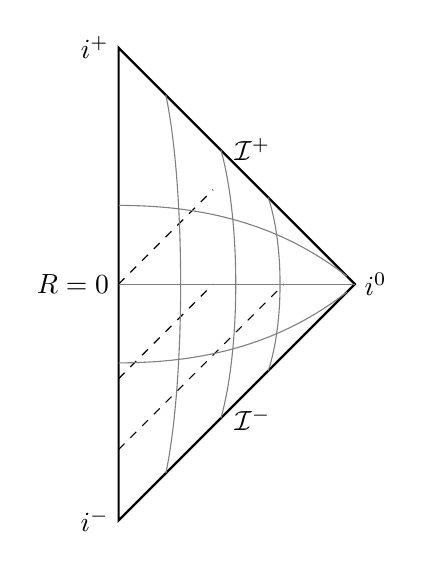
\begin{tikzpicture}[scale=1.0]
\draw[thick] (0,-3) -- (0,3) -- (3,0) -- cycle;

\node[left] at (0,3) {$i^+$};
\node[left] at (0,-3) {$i^-$};
\node[right] at (3,0) {$i^0$};
\node[left] at (0,0) {$R=0$};
\node[above right] at (1.35,1.45) {$\mathcal{I}^+$};
\node[below right] at (1.35,-1.45) {$\mathcal{I}^-$};

\draw[dashed] (0,-2.1) -- (2.1,0.0);
\draw[dashed] (0,-1.2) -- (1.2,0.0);
\draw[dashed] (0,0.0) -- (1.2,1.2);

\draw[gray] (0,0) -- (3,0);
\draw[gray] (0,1.0) .. controls (1.0,1.0) and (2.0,0.8) .. (2.9,0.1);
\draw[gray] (0,-1.0) .. controls (1.0,-1.0) and (2.0,-0.8) .. (2.9,-0.1);

\draw[gray] (0.6,-2.4) .. controls (0.85,-1.2) and (0.85,1.2) .. (0.6,2.4);
\draw[gray] (1.3,-1.7) .. controls (1.55,-0.8) and (1.55,0.8) .. (1.3,1.7);
\draw[gray] (1.9,-1.1) .. controls (2.1,-0.5) and (2.1,0.5) .. (1.9,1.1);
\end{tikzpicture}
\caption{径向约化平直时空的彭罗斯图。等时曲线向外延伸至\(i^0\)，而等半径曲线从\(i^-\)上升至\(i^+\)。}
\end{figure}

讲座中最后一点应当牢记。这些图\emph{并不}保持度规大小。它们保持的是因果结构。这才是我们所追求的不变量。

\begin{classroomqa}
\audiencequestion{紧致化后的等时线应当是直线的吗？}
\lecturerresponse{对于所选映射，只有对称切片\(T=0\)是直线。其他等\(T\)曲线会弯曲，其具体形状取决于紧致化函数。极晚的切片越来越靠近上边界，尽管普通时间无界地继续下去。
\lecturetimestamp{00:29:11--00:30:12}}
\end{classroomqa}

\section{紧致化的施瓦茨席尔德几何}

有了平直空间构造，我们现在回到黑洞，再做同样的事情。我们通过引入零坐标并将无限范围压缩到有限图形中来紧致化克鲁斯卡尔几何。讲师将结果描述为对角矩形或类菱形因果图：视界表现为零边界，外部悬停的世界线留在其外，内部区域终止于一个现在在纸面上可见的奇点。

关键的物理要点是，在坠落观察者的经验中，奇点\emph{并不}位于无穷远。一旦越过视界，在撞上奇点之前剩余的固有时是有限的。彭罗斯图使这一点在视觉上不可避免。

视界再次由施瓦茨席尔德条件确定
\begin{equation}
1-\frac{2MG}{r}=0
\qquad \Longleftrightarrow \qquad
r=2MG.
\end{equation}
等式\(r=2MG\)标出了施瓦茨席尔德因子改变符号的半径。

\begin{figure}[htbp]
\centering
\includegraphics[width=0.72\textwidth]{lecture_08_figure_04.png}
\caption{黑板草图，对比形式延拓图景与物理相关的黑洞区域。红色标签\emph{奇点}在黑板上明确标出。}
\lectureframe{00:37:59}
\end{figure}

\begin{figure}[htbp]
\centering
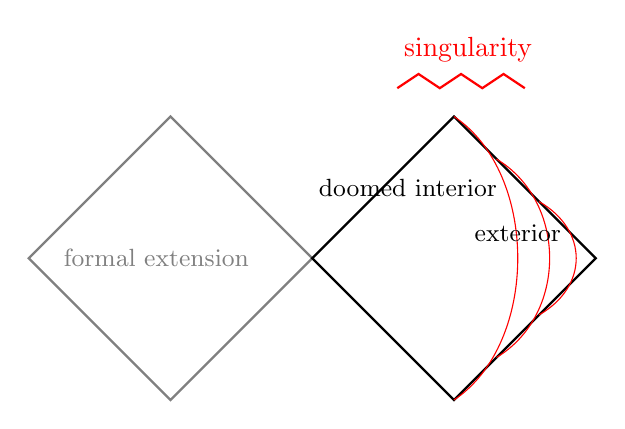
\begin{tikzpicture}[scale=0.9]
\draw[gray,thick] (-4,0) -- (-2,2) -- (0,0) -- (-2,-2) -- cycle;
\draw[thick] (0,0) -- (2,2) -- (4,0) -- (2,-2) -- cycle;

\draw[red,thick] (1.2,2.4) -- (1.5,2.6) -- (1.8,2.4) -- (2.1,2.6) -- (2.4,2.4) -- (2.7,2.6) -- (3.0,2.4);
\node[red] at (2.2,2.95) {singularity};

\draw[red] (2.0,-2.0) .. controls (3.2,-1.2) and (3.2,1.2) .. (2.0,2.0);
\draw[red] (2.6,-1.4) .. controls (3.6,-0.8) and (3.6,0.8) .. (2.6,1.4);
\draw[red] (3.2,-0.8) .. controls (3.9,-0.4) and (3.9,0.4) .. (3.2,0.8);

\node at (2.9,0.35) {\small exterior};
\node at (1.35,1.0) {\small doomed interior};
\node[gray] at (-2.2,0.0) {\small formal extension};
\end{tikzpicture}
\caption{对讲座中强调的因果图景的保守重绘：幸存的外部、注定毁灭的内部、未来奇点，以及与延拓中额外形式部分的对比。}
\end{figure}

讲座在这里非常直接。如果你在外部，你仍可能逃逸，也可能落入。如果你在内部，你就注定毁灭。该图已经说明了关于未来指向因果运动的一切重要内容。

象限\(III\)和\(IV\)是最大延拓克鲁斯卡尔解的合法部分。区域\(III\)提供了第二个外部，区域\(IV\)是时间反演的黑洞区域。然而，它们并不出现在由坍缩形成的普通黑洞的时空中。延拓解在数学上富有教益，恰恰因为坍缩构造将向我们展示哪些部分必须被丢弃。

\section{空间切片、二维球与爱因斯坦--罗森桥}

现在将紧致化图冻结在一个类空切片上，并问该切片作为\emph{空间}而非时空看起来是什么样子。这正是虫洞图像进入之处，也是空间图景不得被允许超出因果论证之处。

由于角方向已被抑制，径向图的每一点代表一个二维球。在施瓦茨席尔德半径\(r\)处，其面积为
\begin{equation}
A=4\pi r^2.
\end{equation}
因此，一个类空切片是一族二维球，而不仅仅是一条一维曲线。当人们沿切片移动时，它们的大小会改变。

在远处，这些球非常大。当人们向内移动时，其半径缩小，直到在视界处达到最小值，
\begin{equation}
r_{\min}=2MG.
\end{equation}
如果人们继续穿过形式延拓，这些球会再次膨胀，朝向另一个渐近侧。这就是爱因斯坦--罗森桥图景。

\begin{figure}[htbp]
\centering
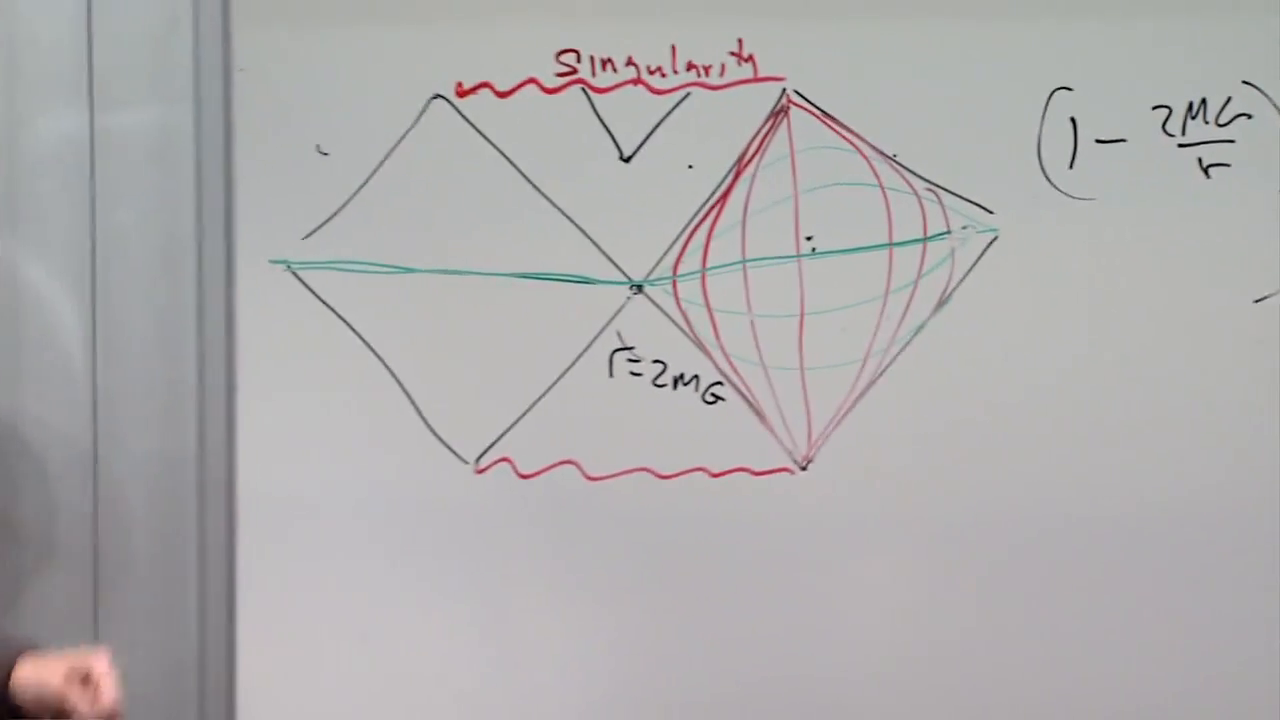
\includegraphics[width=0.72\textwidth]{lecture_08_figure_05.png}
\caption{延拓克鲁斯卡尔图，其中绿色类空切片用于构造桥几何。该切片上的每一点代表一个二维球；其最小半径标为\(r=2MG\)。}
\lectureframe{00:41:30}
\end{figure}

黑板上只显示了相关施瓦茨席尔德因子的一部分，
\begin{equation}
1-\frac{2MG}{r},
\end{equation}
而喉部出现在同一个特殊半径\(r=2MG\)处。

\begin{figure}[htbp]
\centering
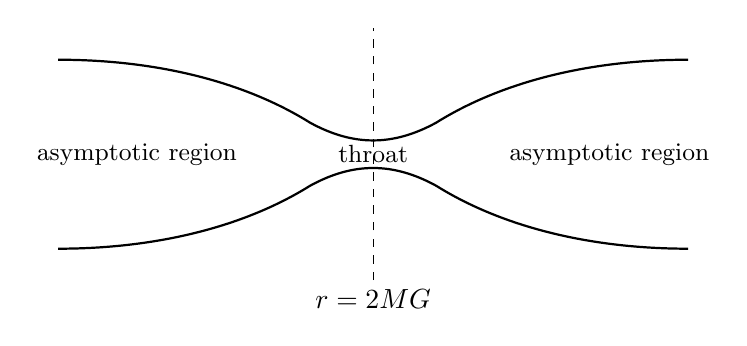
\begin{tikzpicture}[scale=1.0]
\draw[thick] (-4,1.2)
.. controls (-2.7,1.2) and (-1.6,0.9) .. (-0.8,0.4)
.. controls (-0.25,0.1) and (0.25,0.1) .. (0.8,0.4)
.. controls (1.6,0.9) and (2.7,1.2) .. (4,1.2);

\draw[thick] (-4,-1.2)
.. controls (-2.7,-1.2) and (-1.6,-0.9) .. (-0.8,-0.4)
.. controls (-0.25,-0.1) and (0.25,-0.1) .. (0.8,-0.4)
.. controls (1.6,-0.9) and (2.7,-1.2) .. (4,-1.2);

\draw[dashed] (0,-1.6) -- (0,1.6);
\node[below] at (0,-1.6) {$r=2MG$};
\node at (0,0) {\small throat};
\node at (-3.0,0) {\small asymptotic region};
\node at (3.0,0) {\small asymptotic region};
\end{tikzpicture}
\caption{穿过延拓施瓦茨席尔德几何的示意性空间切片。这是对讲座中桥图景的谨慎重建，而非字面嵌入计算。}
\end{figure}

现在来了修正。该切片暗示了两个渐近区域之间的桥，因此诱使人们认为可以通过颈部从一个宇宙旅行到另一个宇宙。讲座先让这一建议出现，然后从因果上将其扼杀。要从一个外部区域到达另一个外部区域，世界线必须在彭罗斯图上的某处变得比\(45^\circ\)零线更浅。这是被禁止的。因此，爱因斯坦--罗森桥是不可穿越的。

讲师还强调了为什么空间图像可能产生误导。它是\emph{某一时刻的空间}的图像；但根本没有足够的因果时间穿过它。可以粗略地说，桥在有任何东西能穿过它之前就打开又关闭了。更好的做法是，直接回头看彭罗斯图，读出因果答案。

\section{从入射零壳构建真实黑洞}

此时讲座完全改变了问题。我们不再读取永恒黑洞的性质。我们正在构建一个真实的黑洞。

选择这个模型是为了简单。我们想象的不是一颗内部结构复杂的坍缩恒星，而是一个薄的球对称入射辐射壳层。它是一个光壳，因此以光速向内运动。在足够小的半径处，该壳层上的能量集中得足够紧密，以至于形成黑洞。

第二个要素是广义相对论形式的壳层定理。

\paragraph{注记。} 对于本讲座中使用的球对称壳层，内部区域是平直时空，而外部区域是史瓦西时空。这就是讲座所使用的可操作的壳层定理，或伯克霍夫型陈述。此处不予证明。

讲师通过首先回顾牛顿壳层定理来引出这一点：在球壳内部没有引力场，而在球壳外部，场与位于中心的点质量的场相同。然后他以这里唯一需要的形式陈述相应的相对论版本：内部是平直的，外部是史瓦西的。壳层可以运动；规则相同。

这足以构建坍缩时空。壳层本身是零的，因此必须画在\(45^\circ\)处。在该零线的一侧，几何是平直的。在另一侧，它是史瓦西的。我们可以将规则总结为
\begin{equation}
\begin{aligned}
\text{inside shell} &= \text{flat spacetime},\\
\text{outside shell} &= \text{Schwarzschild geometry}.
\end{aligned}
\end{equation}

于是粘合方案变得几乎简单得令人尴尬：

\begin{enumerate}
\item 画出平直彭罗斯图，只保留入射壳层内部的区域。
\item 画出史瓦西彭罗斯图，只保留同一壳层外部的区域。
\item 扔掉错误的部分。
\item 将两个保留下来的部分沿壳层轨迹缝合在一起。
\end{enumerate}

这正是讲座在黑板上的做法：丢弃一幅图中错误的一半，丢弃另一幅图中错误的一半，然后沿壳层把正确的两半粘在一起。

\begin{figure}[htbp]
\centering
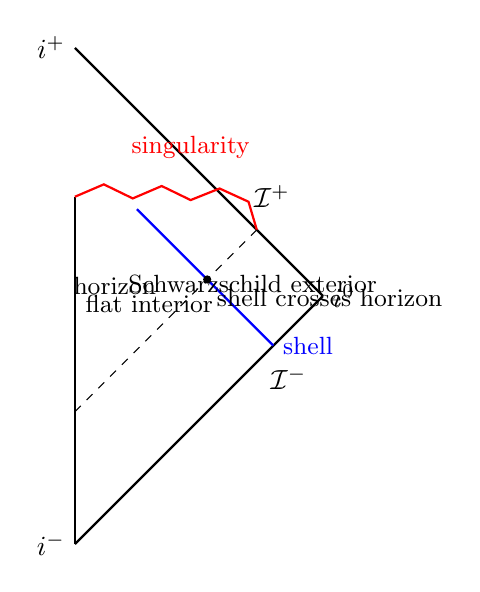
\begin{tikzpicture}[scale=1.05]
\coordinate (im) at (0,-3.0);
\coordinate (ip) at (0,3.0);
\coordinate (i0) at (3.0,0.0);
\coordinate (S)  at (0,1.2);
\coordinate (E)  at (2.2,0.8);
\coordinate (P)  at (2.4,-0.6);
\coordinate (Q)  at (0.75,1.05);
\coordinate (H)  at (0,-1.4);
\coordinate (X)  at (1.6,0.2);

\draw[thick] (im) -- (S);
\draw[thick] (im) -- (i0);
\draw[thick] (ip) -- (i0);

\draw[red,thick] (S) -- (0.35,1.35) -- (0.7,1.18) -- (1.05,1.33) -- (1.4,1.16) -- (1.75,1.30) -- (2.1,1.14) -- (E);
\node[red,above] at (1.4,1.55) {\small singularity};

\draw[thick,blue] (P) -- (Q);
\node[blue,right] at (P) {\small shell};

\draw[dashed] (H) -- (E);
\node[above left] at (1.1,-0.1) {\small horizon};

\filldraw (X) circle (1.2pt);
\node[below right] at (X) {\small shell crosses horizon};

\node at (0.9,-0.1) {\small flat interior};
\node at (2.15,0.15) {\small Schwarzschild exterior};

\node[left] at (im) {$i^-$};
\node[left] at (ip) {$i^+$};
\node[right] at (i0) {$i^0$};
\node[below right] at (2.25,-0.75) {$\mathcal{I}^-$};
\node[above right] at (2.05,0.95) {$\mathcal{I}^+$};
\end{tikzpicture}
\caption{坍缩几何的因果重构。壳层是一条入射零线；在其内部一侧保留平直时空，在其外部一侧保留史瓦西几何。}
\end{figure}

\begin{figure}[htbp]
\centering
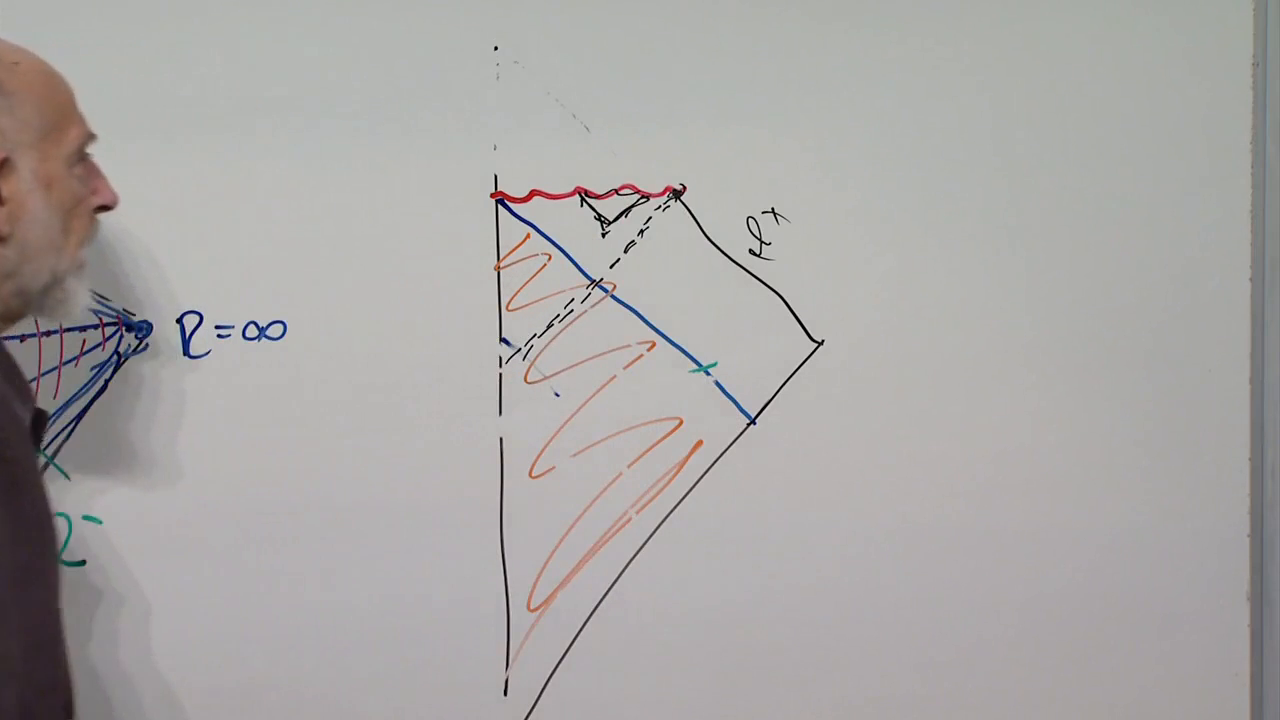
\includegraphics[width=0.76\textwidth]{lecture_08_figure_06.png}
\caption{在平直内部和史瓦西外部沿蓝色入射壳层粘合之后完成的黑板构建。虚线\(45^\circ\)线正从奇点的未来端点向后追踪，以定位事件视界。}
\lectureframe{00:57:30}
\end{figure}

当壳层仅仅从图的平直部分进入史瓦西部分时，壳层本身并没有经历任何特殊的事情。它是一个类光壳层，并继续向内直到到达奇点。本质结构并非由壳层上的局部戏剧性事件承载；它由粘合时空的因果组织承载。

\begin{classroomqa}
\audiencequestion{当坍缩壳层穿过其史瓦西半径时，是否存在不连续性？}
\lecturerresponse{不。在那次穿越中，局部没有发生任何奇异的事情。壳层继续沿其零轨迹运动。特殊事件是因果性的：在壳层穿过其自身的\(2MG\)半径之后，任何未来指向的路径都无法使它返回无穷远。
\lecturetimestamp{00:56:19--00:56:42}}
\end{classroomqa}

\section{到达之前的地平线：事件视界之谜}

现在是讲座的概念高潮。一旦构建了坍缩时空，自然的问题就是：视界在哪里？或者，正如讲师所说，不归点在哪里？

\paragraph{定义。} 事件视界是那些仍能向\(\mathcal{I}^+\)发送未来指向因果信号的事件与那些不能的事件之间的边界。

讲座通过图找到它。从奇点与未来零无穷相交的角点开始，向后追踪一条\(45^\circ\)零线。那条向后追踪的零线就是事件视界。

但讲师随后坚持第二点，而正是这一点让学生们感到不安。视界并非仅仅在壳层穿过其自身施瓦西半径的那一刻出现，然后就固定不动。在放大的黑板图中，视界起初是靠近中心的一个微小 trapped region，向外扩展，穿过一部分仍然平坦的时空，直到后来才与入射壳层相遇。在那个相遇事件处，壳层穿过了它自己的施瓦西半径。在该事件之上，视界就是已形成黑洞的普通的恒定半径视界。

\begin{figure}[htbp]
\centering
\resizebox{0.96\linewidth}{!}{%
\begin{tikzpicture}[scale=1.08,>=Latex]
\coordinate (im) at (0,-3.0);
\coordinate (ip) at (0,3.0);
\coordinate (i0) at (3.0,0.0);
\coordinate (S)  at (0,1.2);
\coordinate (E)  at (2.2,0.8);
\coordinate (P)  at (2.4,-0.6);
\coordinate (Q)  at (0.75,1.05);
\coordinate (H)  at (0,-1.4);
\coordinate (X)  at (1.6,0.2);

\draw[thick] (im) -- (S);
\draw[thick] (im) -- (i0);
\draw[thick] (ip) -- (i0);

\draw[red,thick] (S) -- (0.35,1.35) -- (0.7,1.18) -- (1.05,1.33) -- (1.4,1.16) -- (1.75,1.30) -- (2.1,1.14) -- (E);
\node[red,above left] at (S) {\small singularity};

\draw[very thick,red] (H) -- (E);

\draw[thick,blue] (P) -- (Q);

\filldraw (X) circle (1.2pt);

\draw[gray] (0.0,-2.1) .. controls (0.85,-1.95) and (1.9,-1.3) .. (2.8,-0.2);
\draw[gray] (0.0,-1.2) .. controls (0.95,-1.0) and (1.8,-0.45) .. (2.45,0.35);
\draw[gray] (0.0,-0.2) .. controls (0.8,-0.05) and (1.45,0.35) .. (1.95,0.95);

\node[below right] at (2.28,-0.72) {$\mathcal{I}^-$};
\node[above right] at (2.12,0.92) {$\mathcal{I}^+$};

\draw[very thick,red] (3.2,-1.15) -- (3.75,-1.15);
\node[anchor=west] at (3.85,-1.15) {\small event horizon};
\draw[thick,blue] (3.2,-1.55) -- (3.75,-1.55);
\node[anchor=west] at (3.85,-1.55) {\small infalling shell};
\filldraw (3.48,-1.95) circle (1.2pt);
\node[anchor=west] at (3.85,-1.95)
  {\small shell reaches \(r=2MG\)};
\end{tikzpicture}
}
\caption{强调反向追踪事件视界的坍缩图。视界的一部分位于一个仍然局部平坦、且尚未被壳层到达的区域中。}
\end{figure}

这就是本讲其余部分所详述的引人注目的效应。视界的一部分位于平坦时空中。壳层尚未到达那里，它甚至不在观察者的过去光锥上可见。观察者感受不到引力场，然而却无法逃脱。原因不是局部力。它是该事件的整体因果未来。

\begin{classroomqa}
\audiencequestion{这个构造是说人不能穿过壳层，还是说人不能穿过视界？当壳层的视界仍在其内部时，壳层在哪里？}
\lecturerresponse{人可以穿过壳层。视界是一个不同的零曲面：它是能与\(\mathcal I^+\)通信的事件和不能与之通信的事件之间的边界。入射壳层正是在穿过与其总能量相关联的施瓦茨席尔德半径时遇到该边界。相遇之前，事件视界的一部分穿过平坦的内部；相遇之后，壳层位于已完成的黑洞内部。
\lecturetimestamp{00:58:42--01:01:06}}
\end{classroomqa}

\begin{classroomqa}
\audiencequestion{如果内部是平坦的，而壳层仍然很远，为什么一个刚好在视界内部的人不能在壳层到达之前走过视界？}
\lecturerresponse{画出最快的可能向外的世界线，一条\(45^\circ\)光线。从一个位于反向追踪视界内部的事件出发，即使那条光线也会太晚遇到入射壳层，并终结于奇点。行走还要更慢。\emph{壳层尚未穿过}这一说法在选择一个时间坐标之前是不完整的；因果图给出了与坐标无关的答案。入射的宇宙微波背景不是同一个例子，因为它不是一个产生这种几何的坍缩球壳。
\lecturetimestamp{01:01:07--01:04:03}}
\end{classroomqa}

\section{镜面与改变未来的尝试}

这些问题现在把图变成了一个实验室。假设一个入射光壳层在被困住之前能够被反射。那么所假设的坍缩历史就会改变，事件视界也会改变。这并不矛盾：事件视界只有在完整的时空历史被指定之后才被定义。

\begin{classroomqa}
\audiencequestion{如果把一面完美反射镜放在假定的施瓦西半径之外一点点，使壳层反弹出去，会怎样？}
\lecturerresponse{在那个理想化的历史中，入射零线在镜面处转向外，并到达未来边界；原图中的黑洞不会形成。真正无重量的镜子是不可能的，而物理的镜子会贡献它自身的应力-能量，但这个思想实验说明了逻辑要点：只有在壳层穿过实际的事件视界之后，逃脱才不再可能。
\lecturetimestamp{01:04:33--01:05:54}}
\end{classroomqa}

\begin{classroomqa}
\audiencequestion{一个知道壳层即将到来的观察者能否迅速发出镜子或信号使它转向？}
\lecturerresponse{只有当必要的装置能够足够早地放置在视界之外时才行。Alice 可以事先安排 Bob 发送壳层，因此可以在看到它之前就知道什么即将到来。然而，一旦她的事件位于视界内部，镜子或指令都无法及时到达所需的外部点。对未来实验的知识不会打开图所禁止的因果路径。
\lecturetimestamp{01:05:55--01:08:18}}
\end{classroomqa}

\begin{classroomqa}
\audiencequestion{对于已经位于视界内部的镜子会发生什么？奇点是否在其未来无限远处？}
\lecturerresponse{镜子不过是另一个注定毁灭的物体。它可以在局部反射光，但被反射的光、镜子以及Alice最终都终结于奇点。一条一般的下落世界线在有限的固有时内到达奇点。只有紧致化图中理想的上角才是无限远的。试图停留在那个角附近将需要无界的加速度和能量；此外，在固定事件之间，加速的时钟积累的固有时比惯性时钟更少，而不是更多。
\lecturetimestamp{01:08:19--01:10:19}}
\end{classroomqa}

\begin{classroomqa}
\audiencequestion{如果坍缩的壳层非常巨大，那么位于壳层内部但远离其最终中心的人能否在壳层经过时只是停留在那里？}
\lecturerresponse{可以，只要此人的事件仍然在事件视界之外。位于物质壳层内部与位于黑洞内部不是一回事。辐射可能击中并伤害观察者，但那是与壳层的局部相互作用，与逃逸的因果问题无关。
\lecturetimestamp{01:10:21--01:11:24}}
\end{classroomqa}

\section{时间切片与增长的视界}

弯曲时空中的一个\emph{时间瞬间}意味着一个选定的类空超曲面。这样一组曲面构成一个叶状结构，给每个曲面赋予一个数就定义了一个时间坐标。不同的叶状结构以不同方式切割同一个坍缩图。它们对于哪些遥远事件是同时的持不同意见，但它们不改变哪些零射线到达无穷远。

\begin{figure}[htbp]
\centering
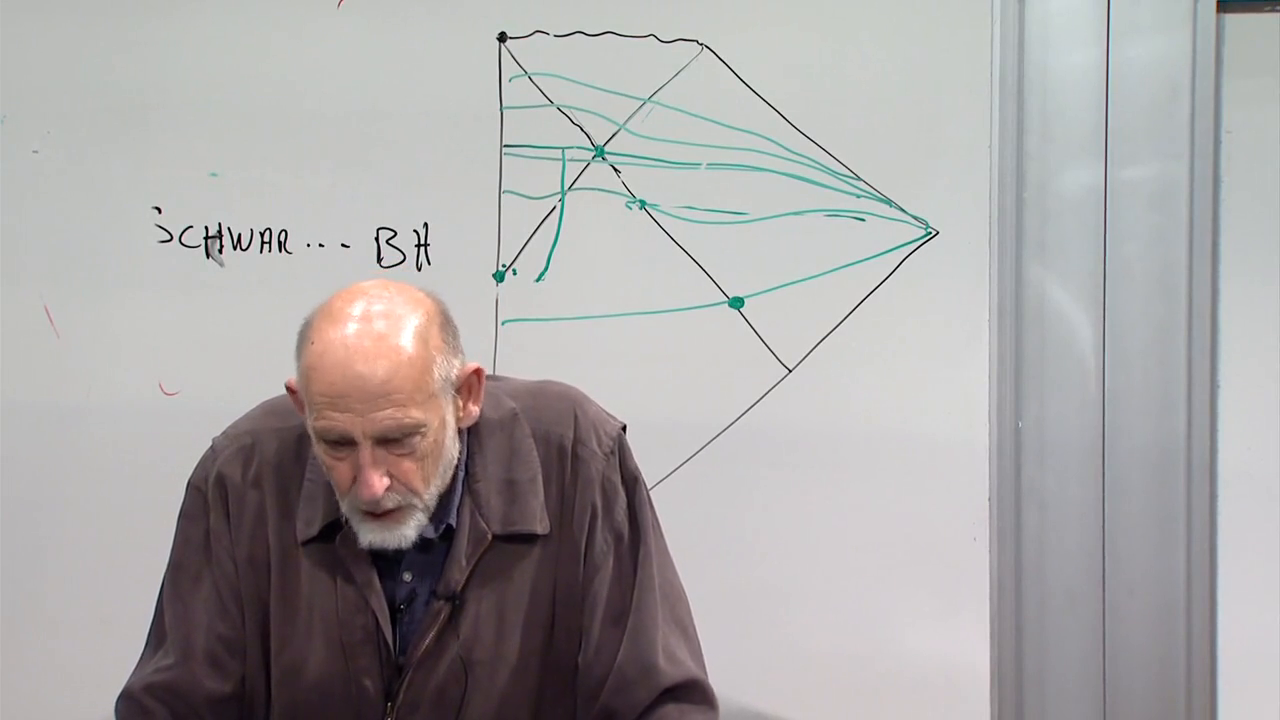
\includegraphics[width=0.77\textwidth]{lecture_08_figure_07.png}
\caption{后期黑板图，带有若干绿色类空切片。这些切片提供了一个时间坐标；黑色零边界及其因果关系独立于该选择。}
\lectureframe{01:17:30}
\end{figure}

\begin{classroomqa}
\audiencequestion{能否通过在一个瞬间比较观察者到视界的距离与视界到壳层的距离来重新表述这个谜题？}
\lecturerresponse{在选定叶状结构之后，这可以是一种有用的直觉，但\emph{在一个瞬间}这个说法依赖于坐标。干净的做法是画出一族类空切片。早期的切片遇到一个巨大的壳层，没有困住中心区域；较晚的切片在仍在坍缩的壳层内部遇到增长的视界；有一个特殊的切片穿过壳层越过其自身施瓦西半径的事件。
\lecturetimestamp{01:11:26--01:14:21}}
\end{classroomqa}

\begin{classroomqa}
\audiencequestion{施瓦西半径是否随着视界向外扩展而增长？为什么壳层越过视界之后视界仍继续增长？}
\lecturerresponse{最终的施瓦西半径\(2MG\)是固定的，因为总质量\(M\)是固定的。在早期类空切片上增长的是视界截面的面积半径。它从中心开始，增大直到在\(r=2MG\)处遇到壳层，然后停止。在相遇事件之上，视界是常\(r\)线\(r=2MG\)，尽管紧致化并不会使那条线看起来竖直或度规上均匀。
\lecturetimestamp{01:14:22--01:16:15}}
\end{classroomqa}

\begin{classroomqa}
\audiencequestion{一个最初位于最终施瓦西半径一半处的观察者会发生什么？该观察者难道不应该只在壳层到达时才感受到引力吗？}
\lecturerresponse{正是如此。观察者首先在仍处于平坦时空时越过增长的视界，感受不到突然的力。下落的辐射壳层是物质性的，之后可能被感受到；事件视界则不是。越过它只意味着现在每一条未来指向的因果路径都无法到达无穷远。正是在这个精确的意义上，视界是幽灵般的。
\lecturetimestamp{01:16:17--01:17:45}}
\end{classroomqa}

\begin{classroomqa}
\audiencequestion{一个足够早出发的观察者能否以比增长的视界更快的速度向外移动并逃逸？}
\lecturerresponse{可以。视界之外的事件有出射因果路径通向\(\mathcal I^+\)；视界之内的事件则没有。在选定的切片上，可以将可用的径向距离与入射壳层封闭路径之前的时间进行比较，但零线给出了精确的检验。没有观察者会看到物质性的视界向外冲来，因为不存在可看到的局部表面。
\lecturetimestamp{01:17:46--01:18:54}}
\end{classroomqa}

\section{图所保留的内容}

页面上的形状不应被解读为按比例的绘图。一个小角落可能代表时空的无限区域，而一大块可能代表适度的物理间隔。紧致化有意牺牲度规大小以保留零方向。留存下来的是因果：谁能向谁发送信号，哪些事件能影响哪些其他事件，以及哪些世界线被光速极限所困。

\begin{classroomqa}
\audiencequestion{如果这幅图如此严重地扭曲了长度和时间，那么它忠实地表示了什么？}
\lecturerresponse{它表示光线，因而表示因果结构。要定位事件视界，就从未来无穷远反向追踪最后一条出射零测地线。试图从纸面上的表观距离推断答案并不可靠。一旦画出了因果图，关于信号、逃逸和无法返回的问题就有了几何答案，尽管度规尺度已被压缩。
\lecturetimestamp{01:18:56--01:21:45}}
\end{classroomqa}

\begin{classroomqa}
\audiencequestion{要熟练到能凭直觉使用彭罗斯图，需要多长时间？}
\lecturerresponse{不需要很久。实用的方法是画它们、追踪零测地线，并检验可能的世界线，直到因果限制变得熟悉。这里的直觉是通过使用这些图获得的，而不是不借助它们去猜测。
\lecturetimestamp{01:21:49--01:22:05}}
\end{classroomqa}

\begin{classroomqa}
\audiencequestion{这种视觉方法是否与量子力学相反？在量子力学中，数学往往比图像更可靠。}
\lecturerresponse{在很大程度上，是的。广义相对论是经典物理。四维弯曲时空很难按字面想象，彭罗斯图也仍然是抽象的，但它的因果几何能够被画出并探索的程度，远远超过量子力学背后的实在所能达到的程度。这一差别正是这些图如此有力的部分原因。
\lecturetimestamp{01:22:05--01:22:58}}
\end{classroomqa}